\begin{homeworkProblem}[4]
\begin{enumerate}
% 4(a)
\item The relationship between $\lambda$ and $K$ is depicted below in Figure
\ref{fig:fig4a}.
\begin{SCfigure}[4][h]
    \centering
    \caption[The relationship between $\lambda$]{
        The relationship between $\lambda = \exp[r(1-N_t/K)]$ and $K$.
        $\lambda$, the population's growth rate, is described as a function of
        $K$. Here $K$ is selected to be $50$ and $r$ is selected to be $2$.
    }
    \label{fig:fig4a}
    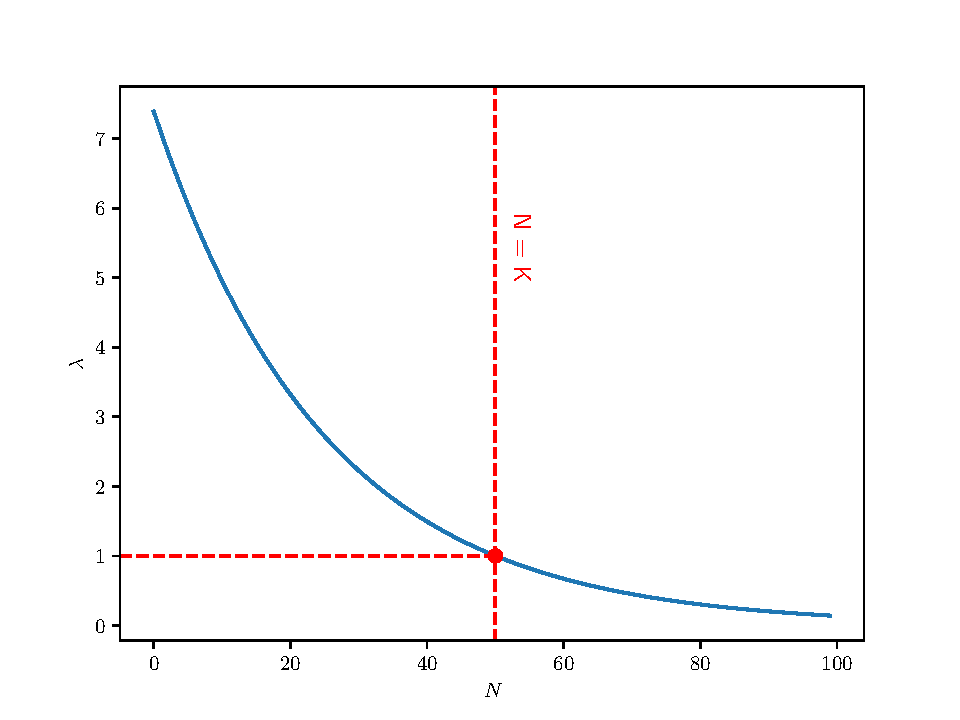
\includegraphics[scale=0.4]{fig/fig4(a).pdf}
\end{SCfigure}
It's clear in Figure \ref{fig:fig4a} that $\lambda > 1$ when $N < K$, i.e., the
population can continue to grow and reproduce only if $N < K$.

% 4(b)
\item Plug in $\bar N = K$ into the equation, we'll have \[
    \begin{aligned}
        N_t &= \bar N = K,\\
        N_{t+1} &= N_t \exp[r(1-N_t/K)] = K \exp[r(1-K/K)] = K
    \end{aligned}
\]
Therefore, for $\bar N$ can make $N_{t+1} = N_t$ for two successive timepoints.
It is indeed the steady state.

% 4(c)
\item The condition of stability for the steady state depends on: \[
    \begin{aligned}
        &\left|\left.\derivlong[N]{N\exp[r(1-N/K)]}\right|_{\bar N}\right|\\
        &\qquad = \left| \left.\left(
            \exp[r(1-N/K)] - \frac{rN}{K} \exp[r(1-N/K)]
        \right)\right|_{\bar N} \right|\\
        &\qquad = |1 - r|
    \end{aligned}
\]
To make the steady state stable, we need \[
    |1-r| < 1
\]
Solving this inequity gives \[
    \begin{aligned}
        0 < r < 2
    \end{aligned}
\]

\pagebreak
% 4(d)
\item See explanation in the figure legends. We've known from (c) that the
stability only depends on $r$ but not $K$, hence I only chose to depict various
$r$ values. In every picture the $K$ is selected to be $200$. And the initial
value is selected to be $5$. A $r$ value smaller than $0$ is not biologically
sensible, hence not
included in the simulation.
\begin{SCfigure}[1][htbp]
    \centering
    \caption{$N_t$ behavior when $r = 0.5$. It's clear that the steady state is
    stable, which confirms the stability condition $0 < r < 2$}
    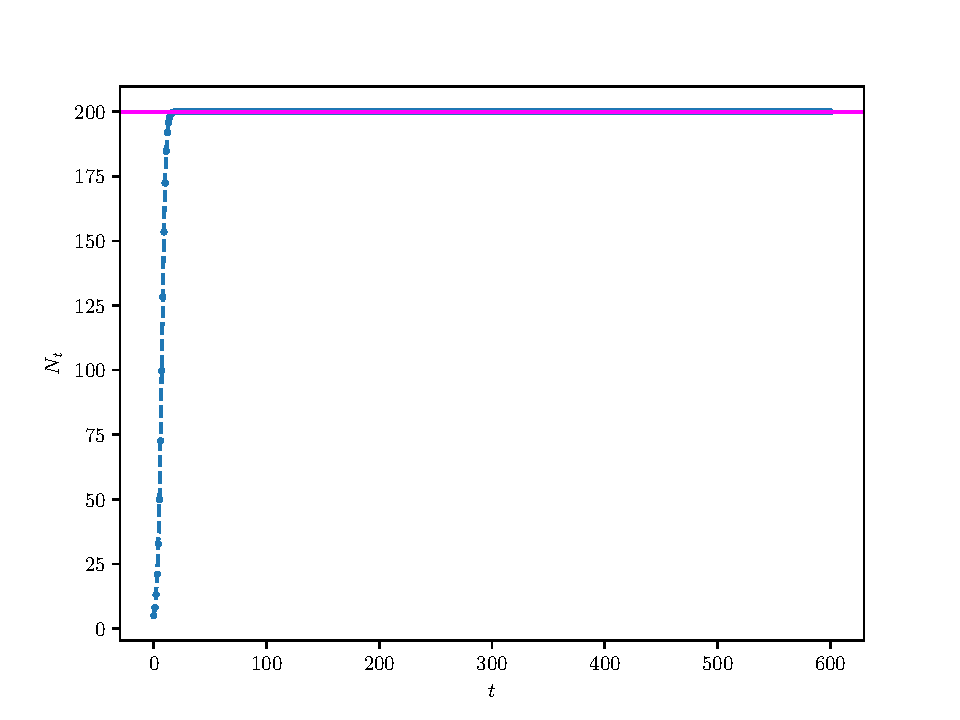
\includegraphics[scale=0.6]{fig/fig4(d)(1).pdf}
\end{SCfigure}
\begin{SCfigure}[2][htbp]
    \centering
    \caption{$N_t$ behavior when $r = 1.0$. It's clear that the steady state is
    still stable, which confirms the stability condition $0 < r < 2$}
    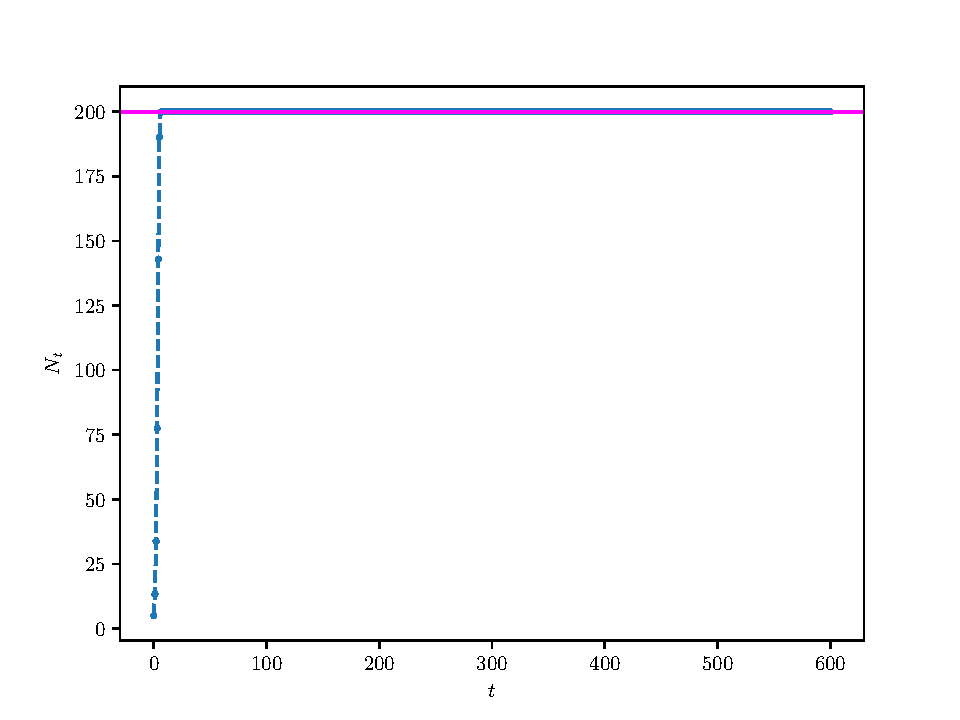
\includegraphics[scale=0.6]{fig/fig4(d)(2).pdf}
\end{SCfigure}
\begin{SCfigure}[3][htbp]
    \centering
    \caption{$N_t$ behavior when $r = 1.5$. It's clear that the steady state is
    still stable, which confirms the stability condition $0 < r < 2$}
    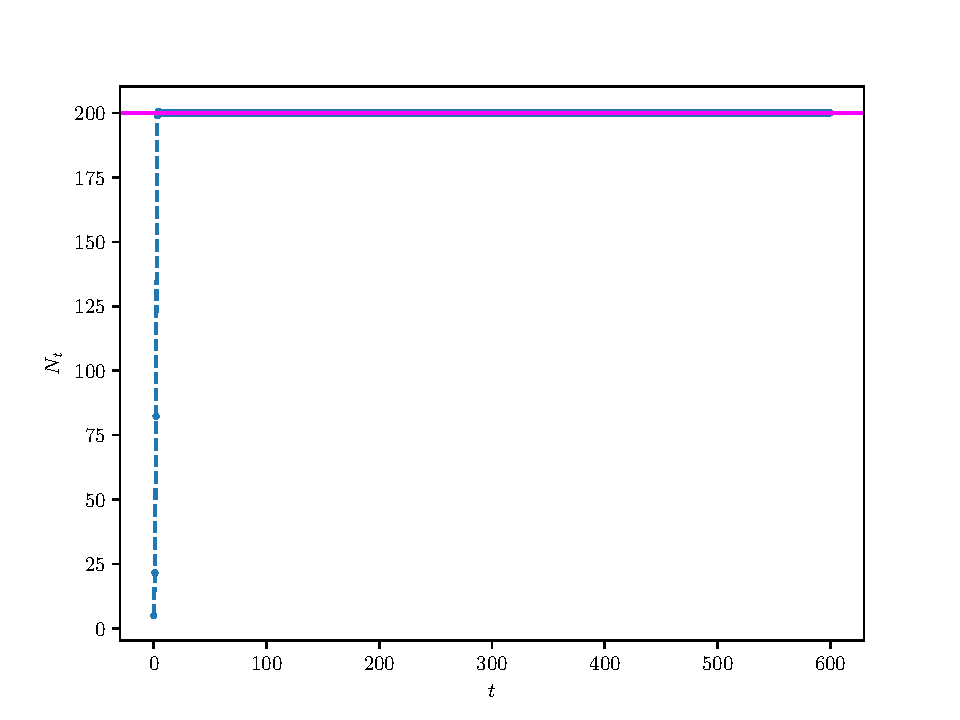
\includegraphics[scale=0.6]{fig/fig4(d)(3).pdf}
\end{SCfigure}
\begin{SCfigure}[4][htbp]
    \centering
    \caption{$N_t$ behavior when $r = 2$, which is the boundary value for
    stability. Moderate oscillation observed around steady state.}
    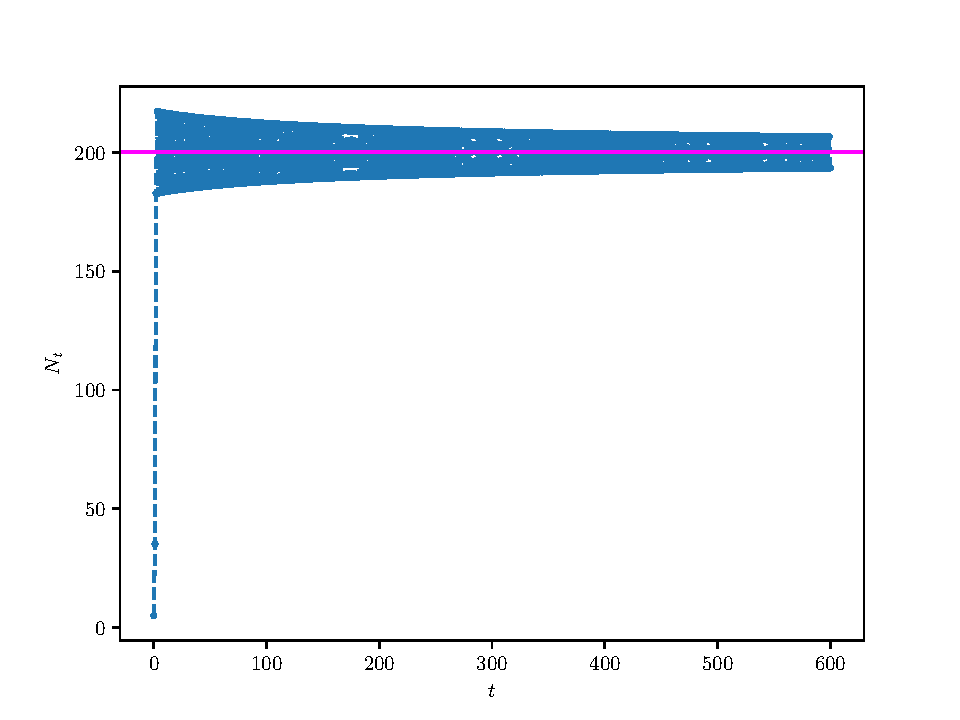
\includegraphics[scale=0.6]{fig/fig4(d)(4).pdf}
\end{SCfigure}

\begin{figure}[htbp]
    \begin{subfigure}[t]{0.4\linewidth}
        \centering
        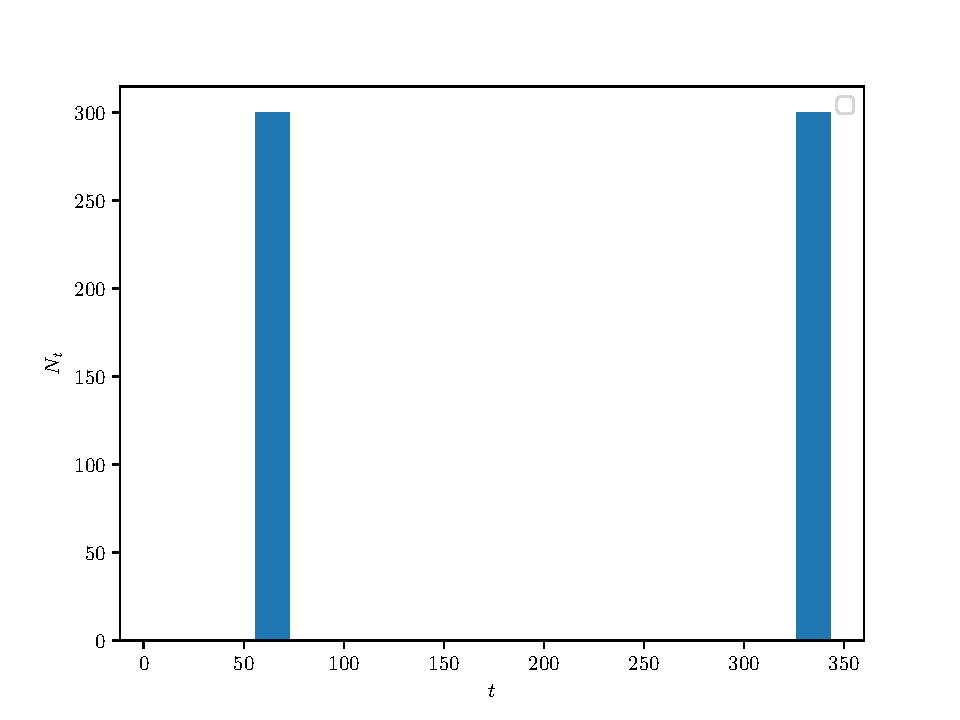
\includegraphics[scale=0.5]{fig/fig4(d)(5).pdf}
        \caption{$N_t$ behavior}
    \end{subfigure}
    \hfill
    \begin{subfigure}[t]{0.4\linewidth}
        \centering
        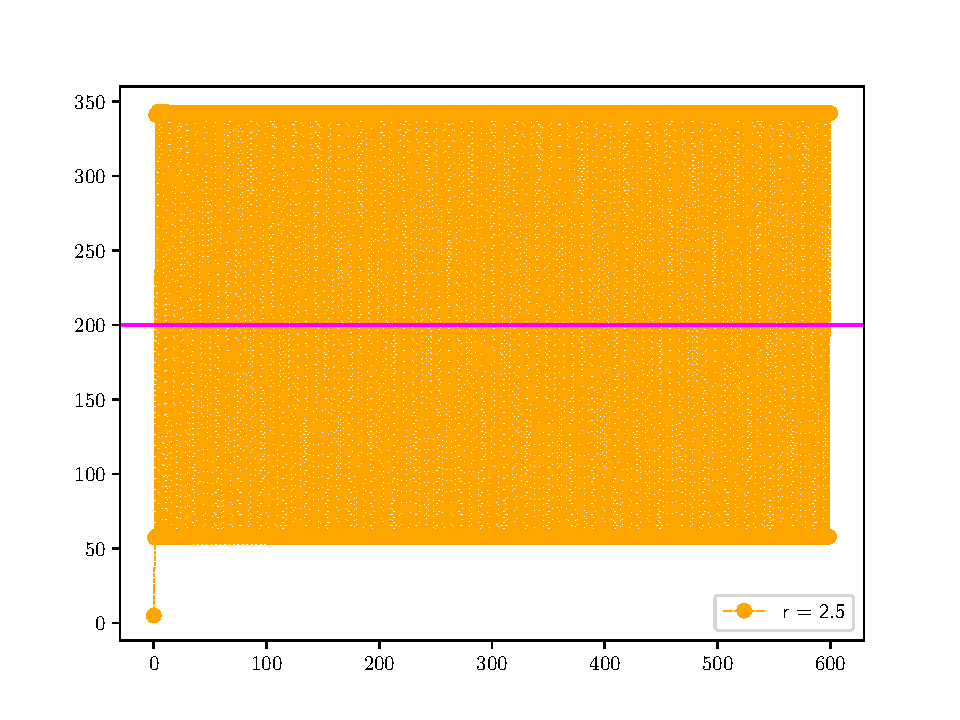
\includegraphics[scale=0.5]{fig/fig4(d)(5)_chaos2.5.pdf}
        \caption{Histogram}
    \end{subfigure}
    \caption{$N_t$ behavior when $r = 2.5$, seemingly chaotic but actually still
    maintains oscillation around the steady state. The histogram can confirm
    that most $N_t$ values fall in the most conspicuous 2 bars (and there's a
    very short bar between 0-50! Those are points before reaching steady state).}
    \label{fig:fig12}
    \vspace*{\floatsep}
    \begin{subfigure}[t]{0.4\linewidth}
        \centering
        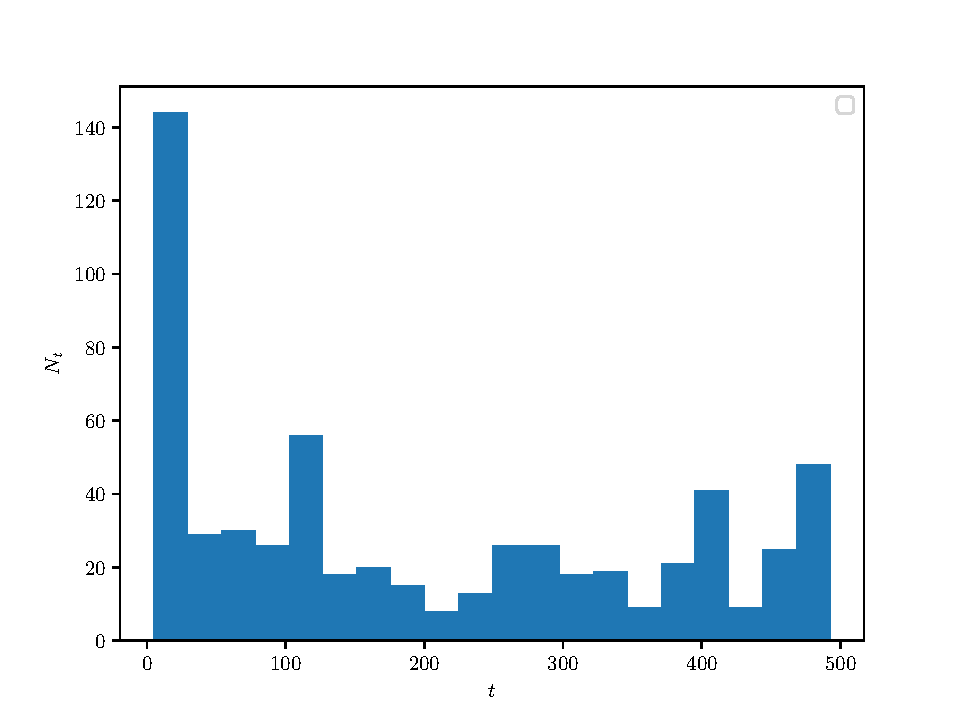
\includegraphics[scale=0.5]{fig/fig4(d)(6).pdf}
        \caption{$N_t$ behavior}
    \end{subfigure}
    \hfill
    \begin{subfigure}[t]{0.4\linewidth}
        \centering
        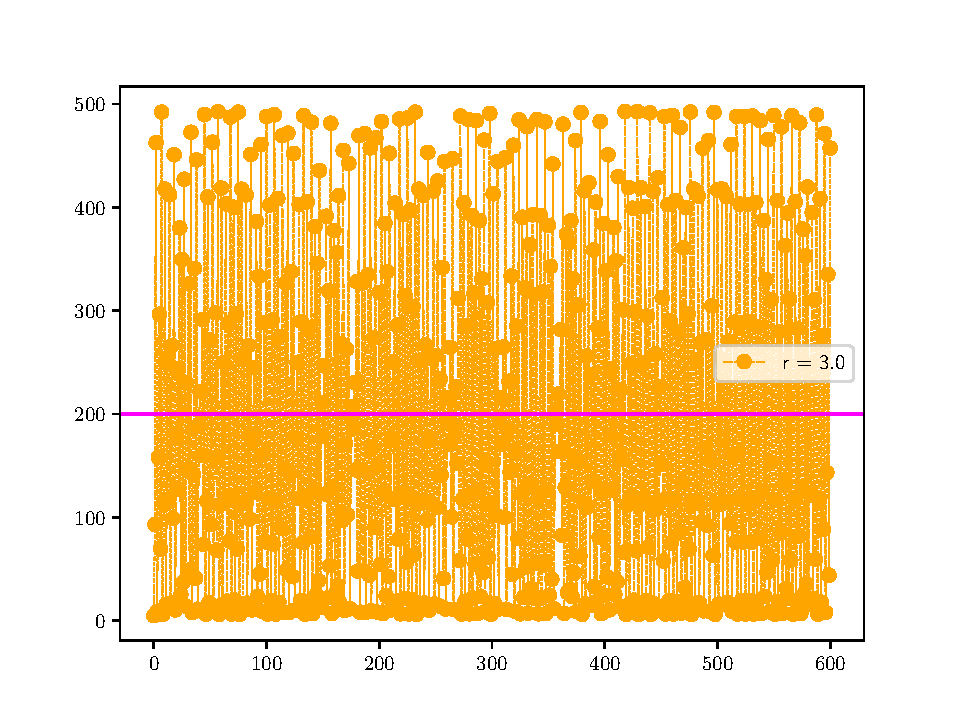
\includegraphics[scale=0.5]{fig/fig4(d)(6)_chaos3.0.pdf}
        \caption{Histogram}
    \end{subfigure}
    \caption{$N_t$ behavior when $r = 3$, truly chaotic. The chaos status can
    be confirmed from the histogram --- it's rather uniformly distributed
    compared to the situation when $r = 2.5$.}
    \label{fig:fig13}
\end{figure}
\pagebreak
\end{enumerate}
\end{homeworkProblem}